%% ============================================================================
\section{Experimental Setup}
\label{sec:setup}
%% ============================================================================

\subsection{Test rig}
\label{subsec:rig}

The test rig is a custom-built bearing test stand at Aarhus University (Herning, Denmark). The rig is used for conducting experiments under conditions, where rotational speed, load, temperature, and lubricant amount can be controlled.

\begin{description}
  \item[\textbf{Bearing:}] a deep-groove ball bearing of model SYJ25 with \SI{25}{mm} bore width, pitch diameter $d_{pw} = \SI{38.0}{mm}$, 9 steel rolling elements, and dynamic load rating \SI{14000}{N}.
  \item[\textbf{Rotational speed:}] the bearing is driven by a Klee T712-2 0.55kW variable-frequency electric motor controlled through a variable-frequency drive (VFD). The VFD is controlled by a PID-controller based on measurements by an OGT5000 diffuse reflection sensor. The VFD switching frequency is nominally 5kHz, and the harmonic artifacts from this are sought filtered out \todo{Explain the filter and how effective it is expected to be.}.
  \item[\textbf{Temperature:}] temperature is increased by a heating element mounted on the bearing pillow block and controlled by an Omron E5CC PID controller based on measurements from a type K temperature sensor mounted on the outer ring of the bearing.
  \item[\textbf{Load:}] the bearing is loaded radially by a static weight of 60kg, and the actual load is measured by an FN2114 pedal load cell.
  \item[\textbf{Lubricant:}] the bearing is lubricated with 0.5ml \todo{Check that this is correct} of Keratech~22 oil (kinematic viscosity $\nu_{40} = \SI{22}{cSt}$, $\nu_{100} = \SI{4.1}{cSt}$ at 40\si{\celsius} and 100\si{\celsius}, respectively) \todo{Do we need NLGI cosistency grade?}.
  \item[\textbf{Acoustic emission sensor:}] A Kistler Piezotron Type~8152C1 wideband piezoelectric AE sensor bonded to the bearing housing. Its output is conditioned by a Kistler Type~5125C AE Piezotron coupler, which powers the sensor and applies a Butterworth band-pass filter from \SI{50}{kHz} to \SI{1}{MHz} to the raw AE signal before it is digitised. This coupler band-pass, sets the \SI{1}{MHz} upper analysis limit used throughout the paper.
  \item[\textbf{Ultrasound sensor:}]
\end{description}

The test rig can be seen in Figure~\ref{fig:test_rig}.

\begin{figure}[H]
\centering
\begin{subfigure}[t]{0.32\textwidth}
  \centering
  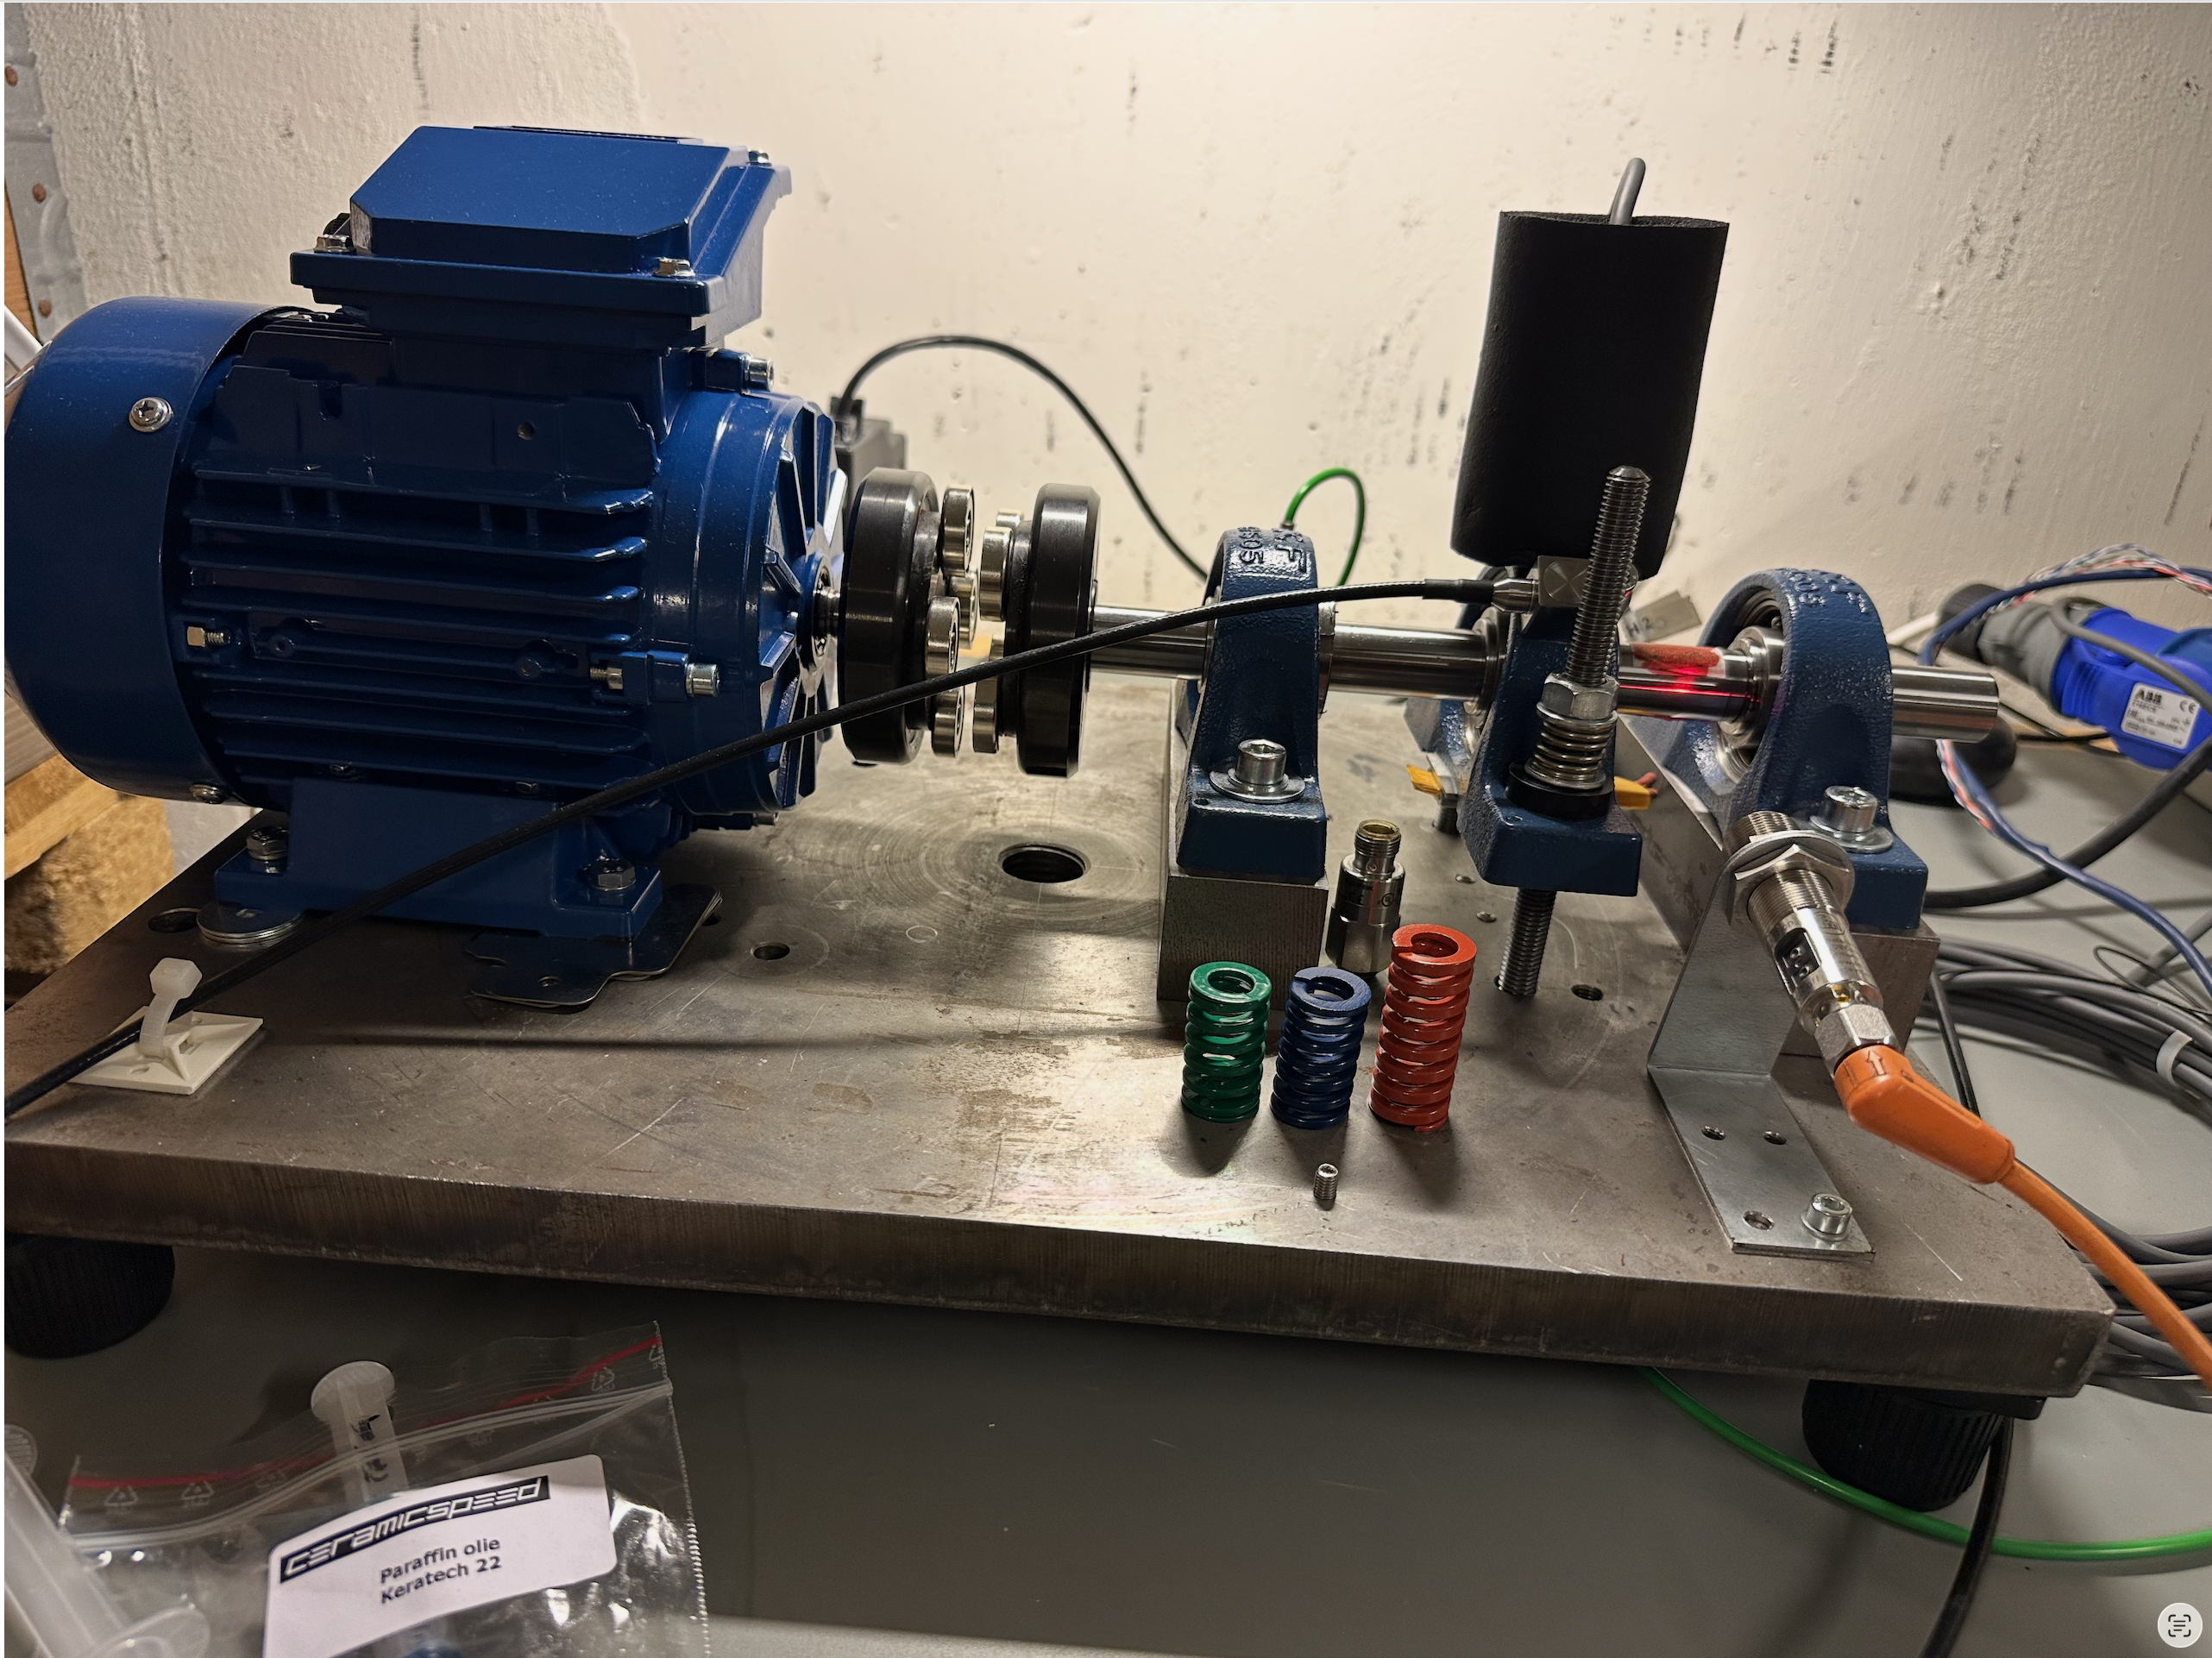
\includegraphics[width=\textwidth]{figures/test_rig_overview.png}
  \caption{}
  \label{fig:rig_overview}
\end{subfigure}\hfill
\begin{subfigure}[t]{0.32\textwidth}
  \centering
  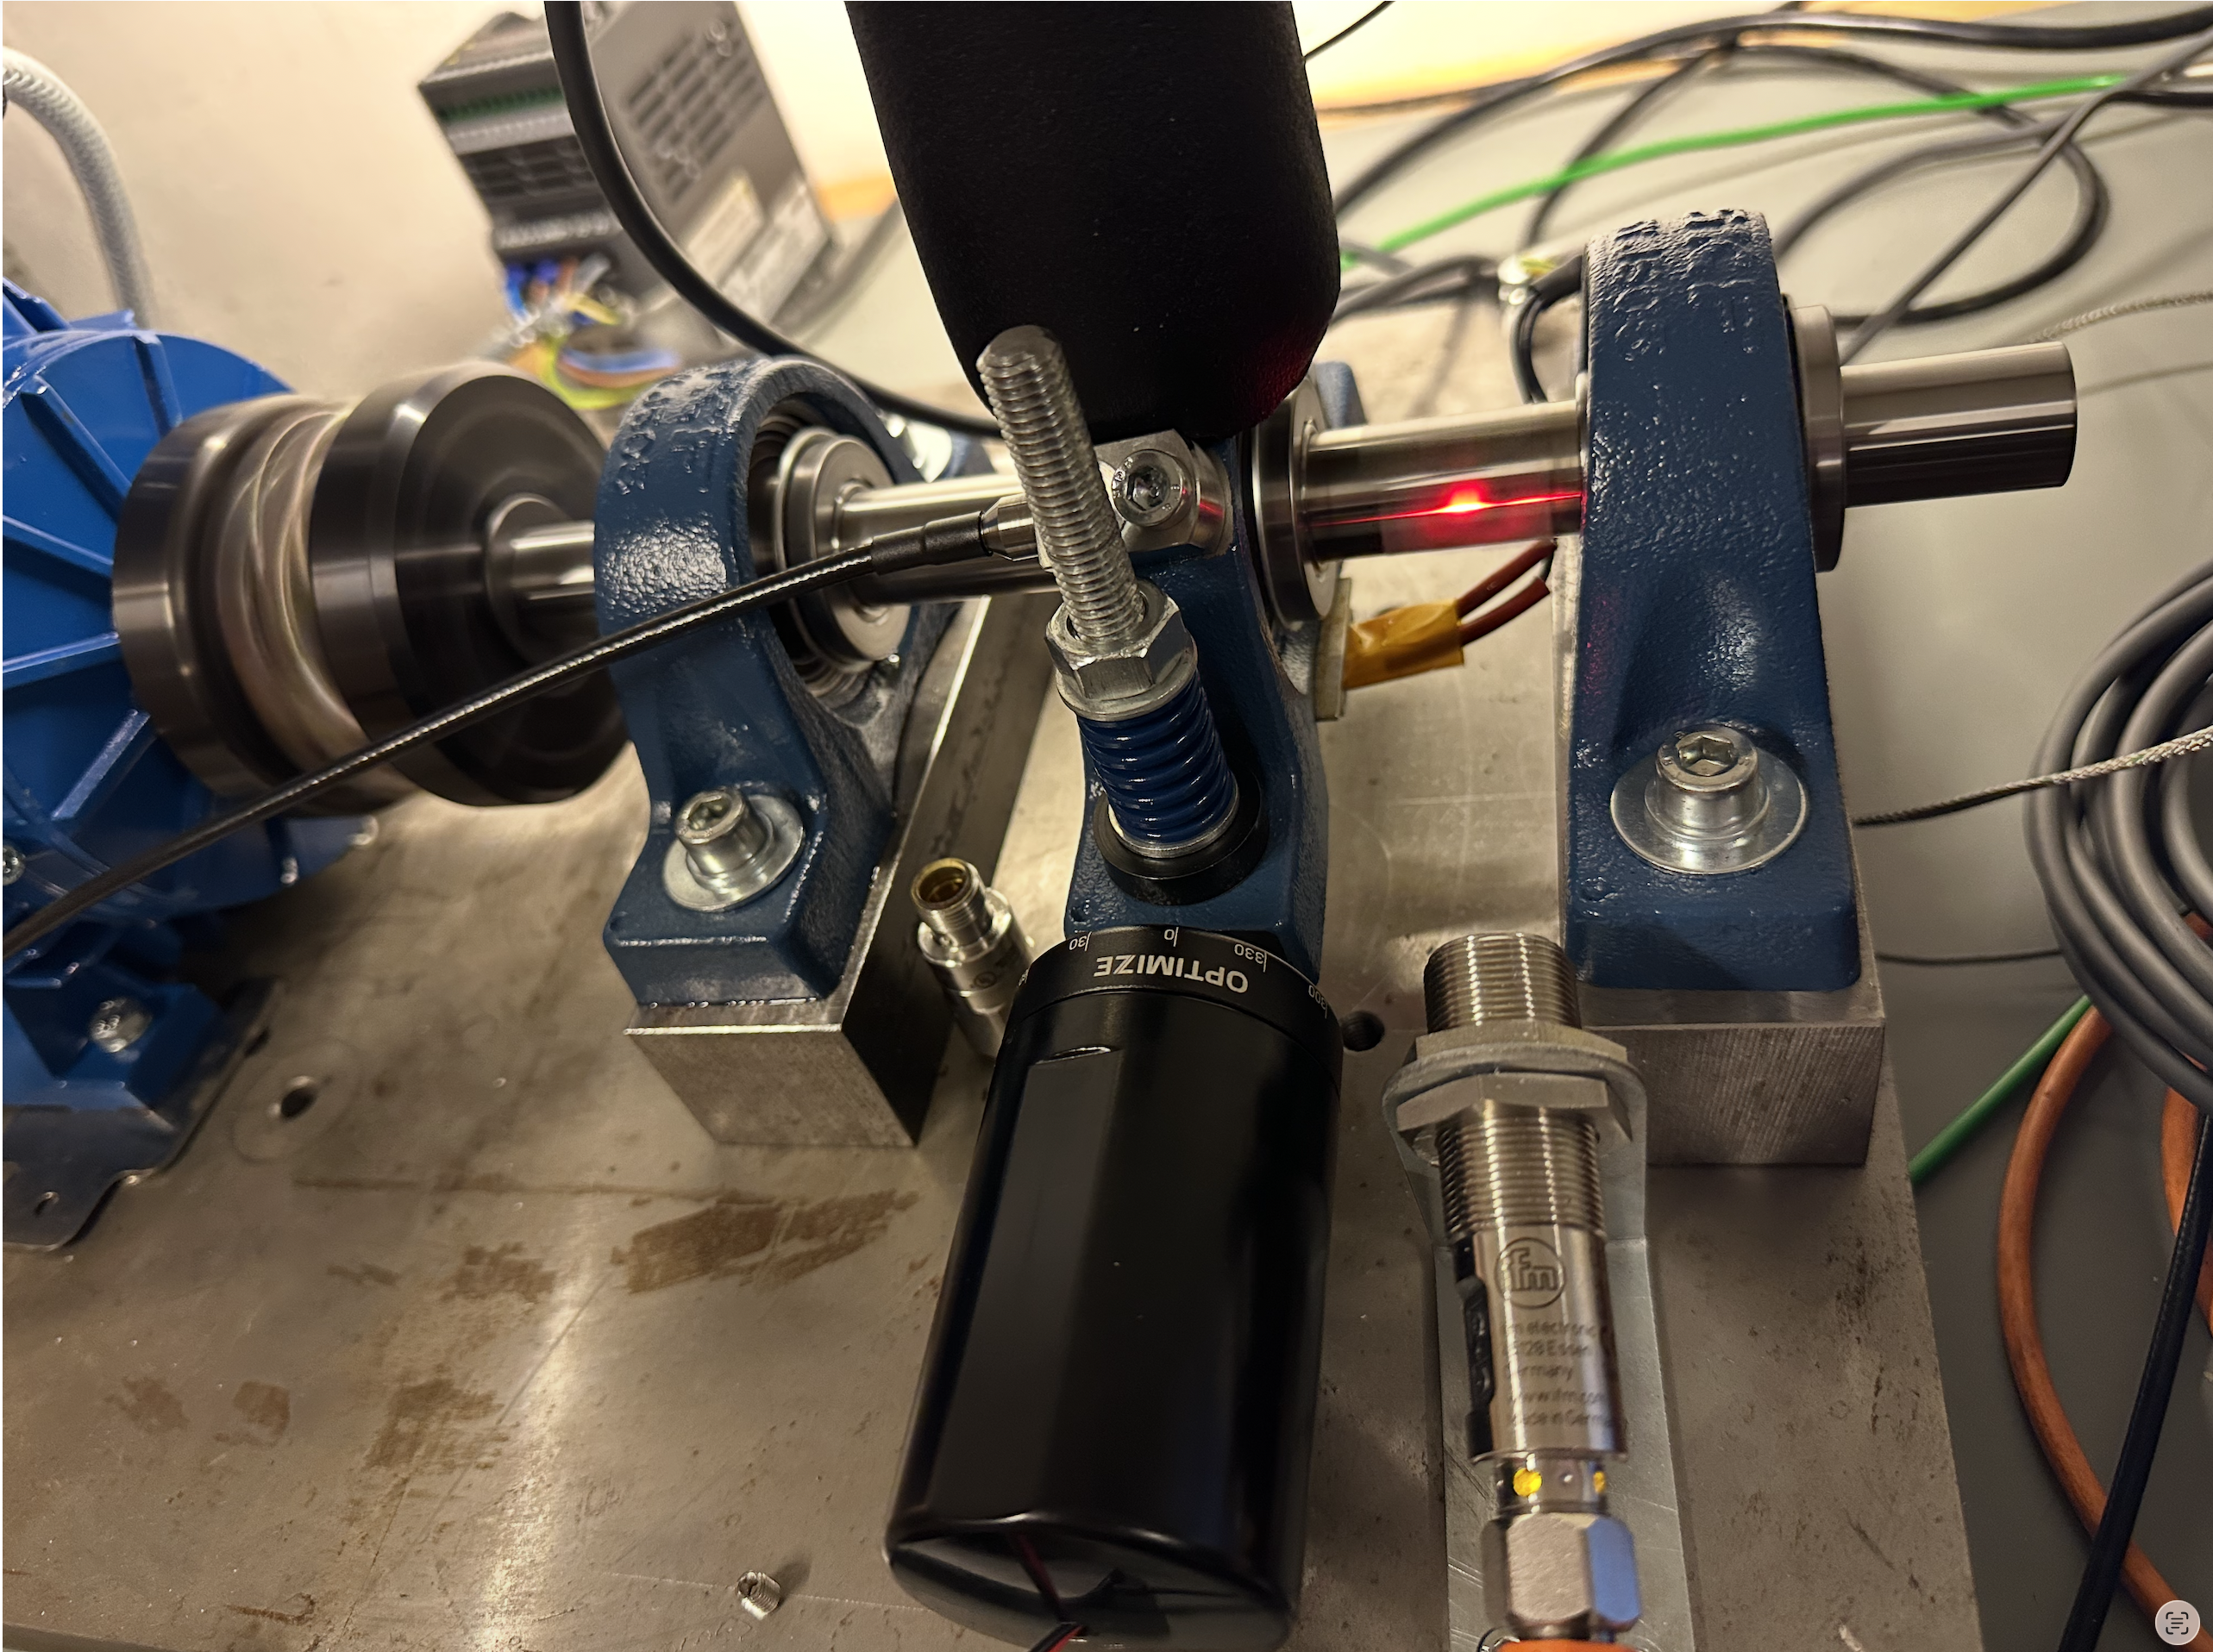
\includegraphics[width=\textwidth]{figures/test_rig_sensors.png}
  \caption{}
  \label{fig:rig_sensors}
\end{subfigure}\hfill
\begin{subfigure}[t]{0.32\textwidth}
  \centering
  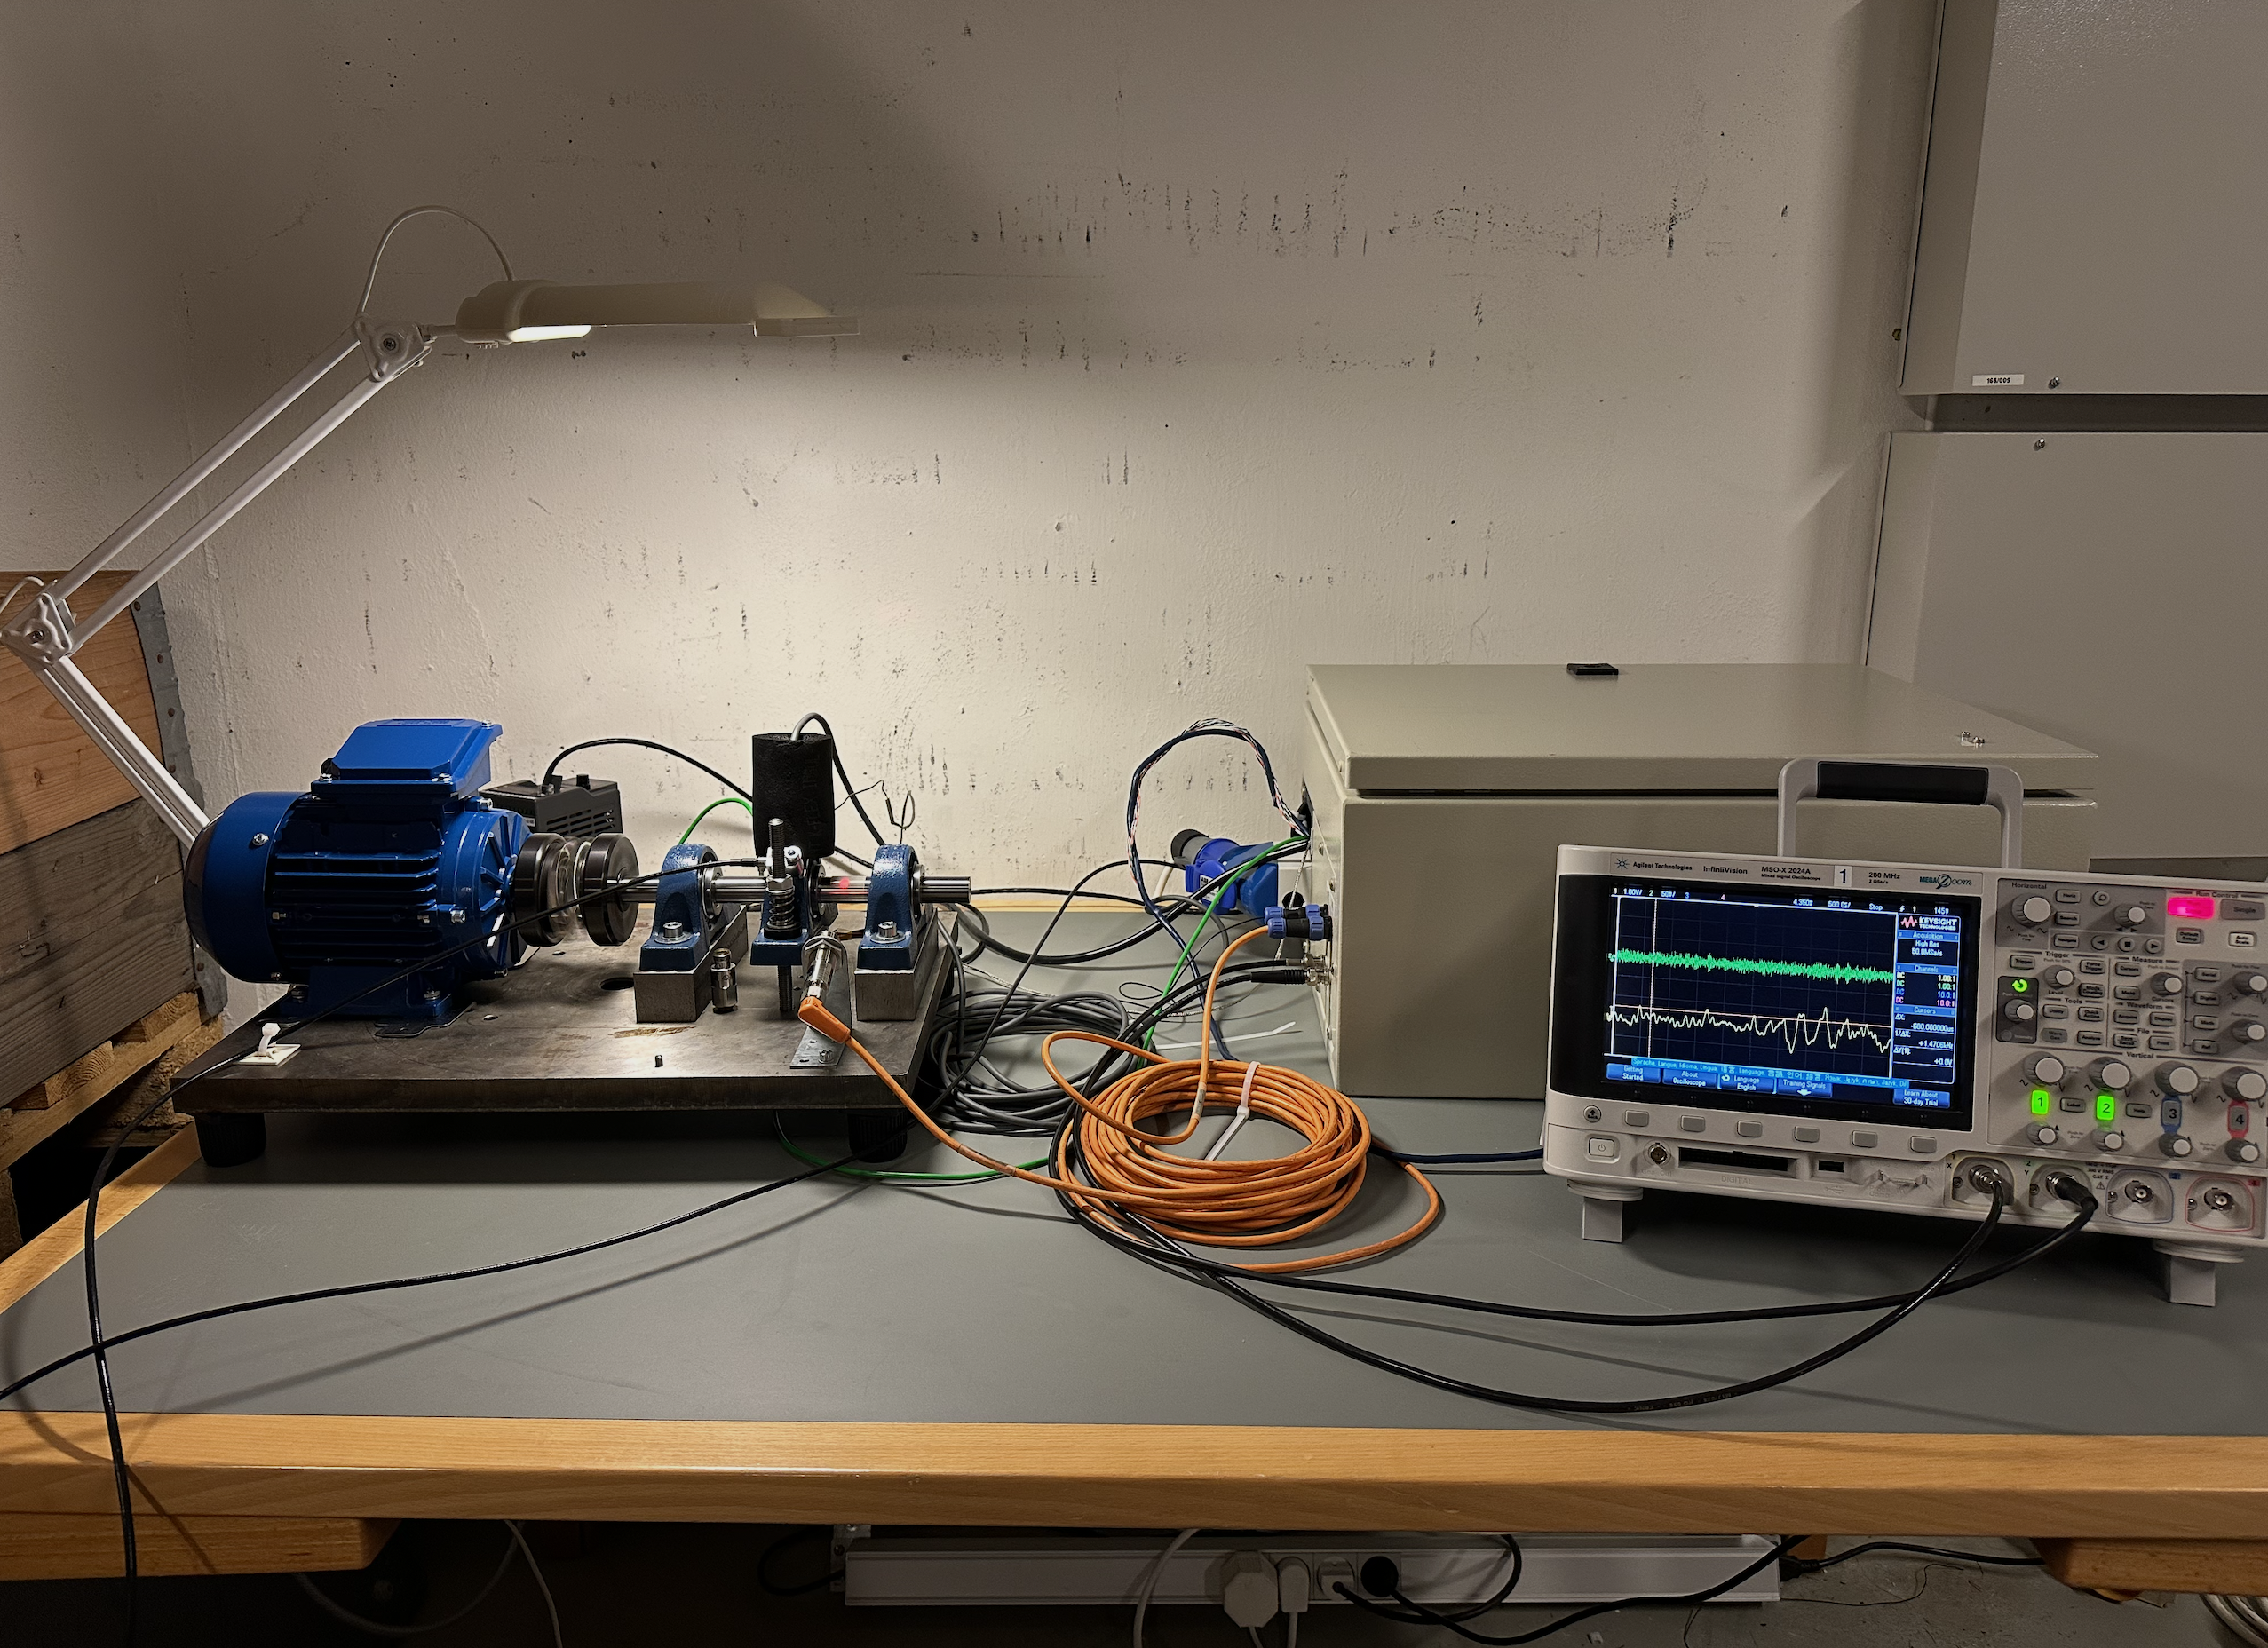
\includegraphics[width=\textwidth]{figures/test_rig_full_setup.png}
  \caption{}
  \label{fig:rig_full_setup}
\end{subfigure}
\caption{The custom-built bearing test rig at Aarhus University (Herning, Denmark).}
\label{fig:test_rig}
\end{figure}\todo{Update figure according to kappa thresholds}

\subsection{Operating condition variation protocol}
\label{subsec:ops}

The experiment follows a protocol which varies the nominal operating conditions through changes in rotational speed (RPM) and housing temperature (\si{\celsius}). This causes the viscosity ratio $\kappa$ of the bearing in the test rig to vary under controlled loading and bearing geometry.

\textbf{Speed:} rotational speed follows a staircase sweep from 100 to 3000 RPM and back down to 100 RPM in steps of 100 RPM with a minimum 60-second hold at each step. This staircase is repeated for 13 temperature blocks.

\textbf{Temperature:} temperature is increased in coherent blocks from 40 to 100~\si{\celsius} in 5~\si{\celsius} increments. After each RPM downsweep from 3000 RPM to 100 RPM, the housing is brought to the next temperature set-point before the next RPM staircase sweep begins.

\textbf{Load:} radial load is applied with a static dead-weight, and held constant throughout the experiment at approximately \SI{61}{kg}.

The hold at the \SI{3000}{rpm} staircase peak is substantially longer than the ordinary 60-second steps (approximately 20~minutes), so this operating point is over-represented in the data: it accounts for roughly a third of all sweeps.\todo{Confirm why the 3000~rpm peak is held for $\sim$20~min (the temperature set-point is not changed there).}  The total duration of the experiment is approximately 14 hours and the measured operating conditions span \resRpmMinMeas--\resRpmMaxMeas~rpm and \resTempMinMeas--\resTempMaxMeas~\si{\celsius}; the measured temperature range extends below the commanded \SI{40}{\celsius} floor (down to $\approx$\SI{33}{\celsius}), which is tentatively attributed to instability of the temperature control rather than to any commanded set-point.

The lubrication conditions in the bearing are not expected to change during the experiment in other ways than what is entailed by rpm and temperature and the effect of these upon the lubricant. It is not expected or assumed that any degradation, starvation or contamination of the lubricant happens.

Since the operating conditions are maintained through a control loop, they vary from the nominal conditions specified by the protocol, and during the last temperature block, the speed recordings at the top of the speed staircase were corrupted and are therefore discarded. The measured operating conditions space and the distribution of calculated $\kappa$ values are seen in Figure~\ref{fig:op_conditions_distribution}. The measured operating conditions over time, ordered by segments are seen in Figure~\ref{fig:op_conditions_timeseries}. The $\kappa$ value for each segment is computed according to Equations~\eqref{eq:kappa} and \eqref{eq:nu1} using the per-segment measured RPM and temperature, with \nuop{} evaluated via the ASTM~D341 Walther equation.

\begin{figure}[H]
\centering

\includegraphics[width=0.9\textwidth]{figures/eda_operating_conditions.png}
\caption{Left: scatterplot of the measured operating conditions (rpm and temperature) during the experiment. Each point corresponds to a 20ms segment of sampling at a given rpm and temperature. The colour of each point corresponds to the derived $\kappa$ value for that segment. Right: distribution of the derived $\kappa$ values.}
\label{fig:op_conditions_distribution}
\end{figure}

\begin{figure}[H]
\centering
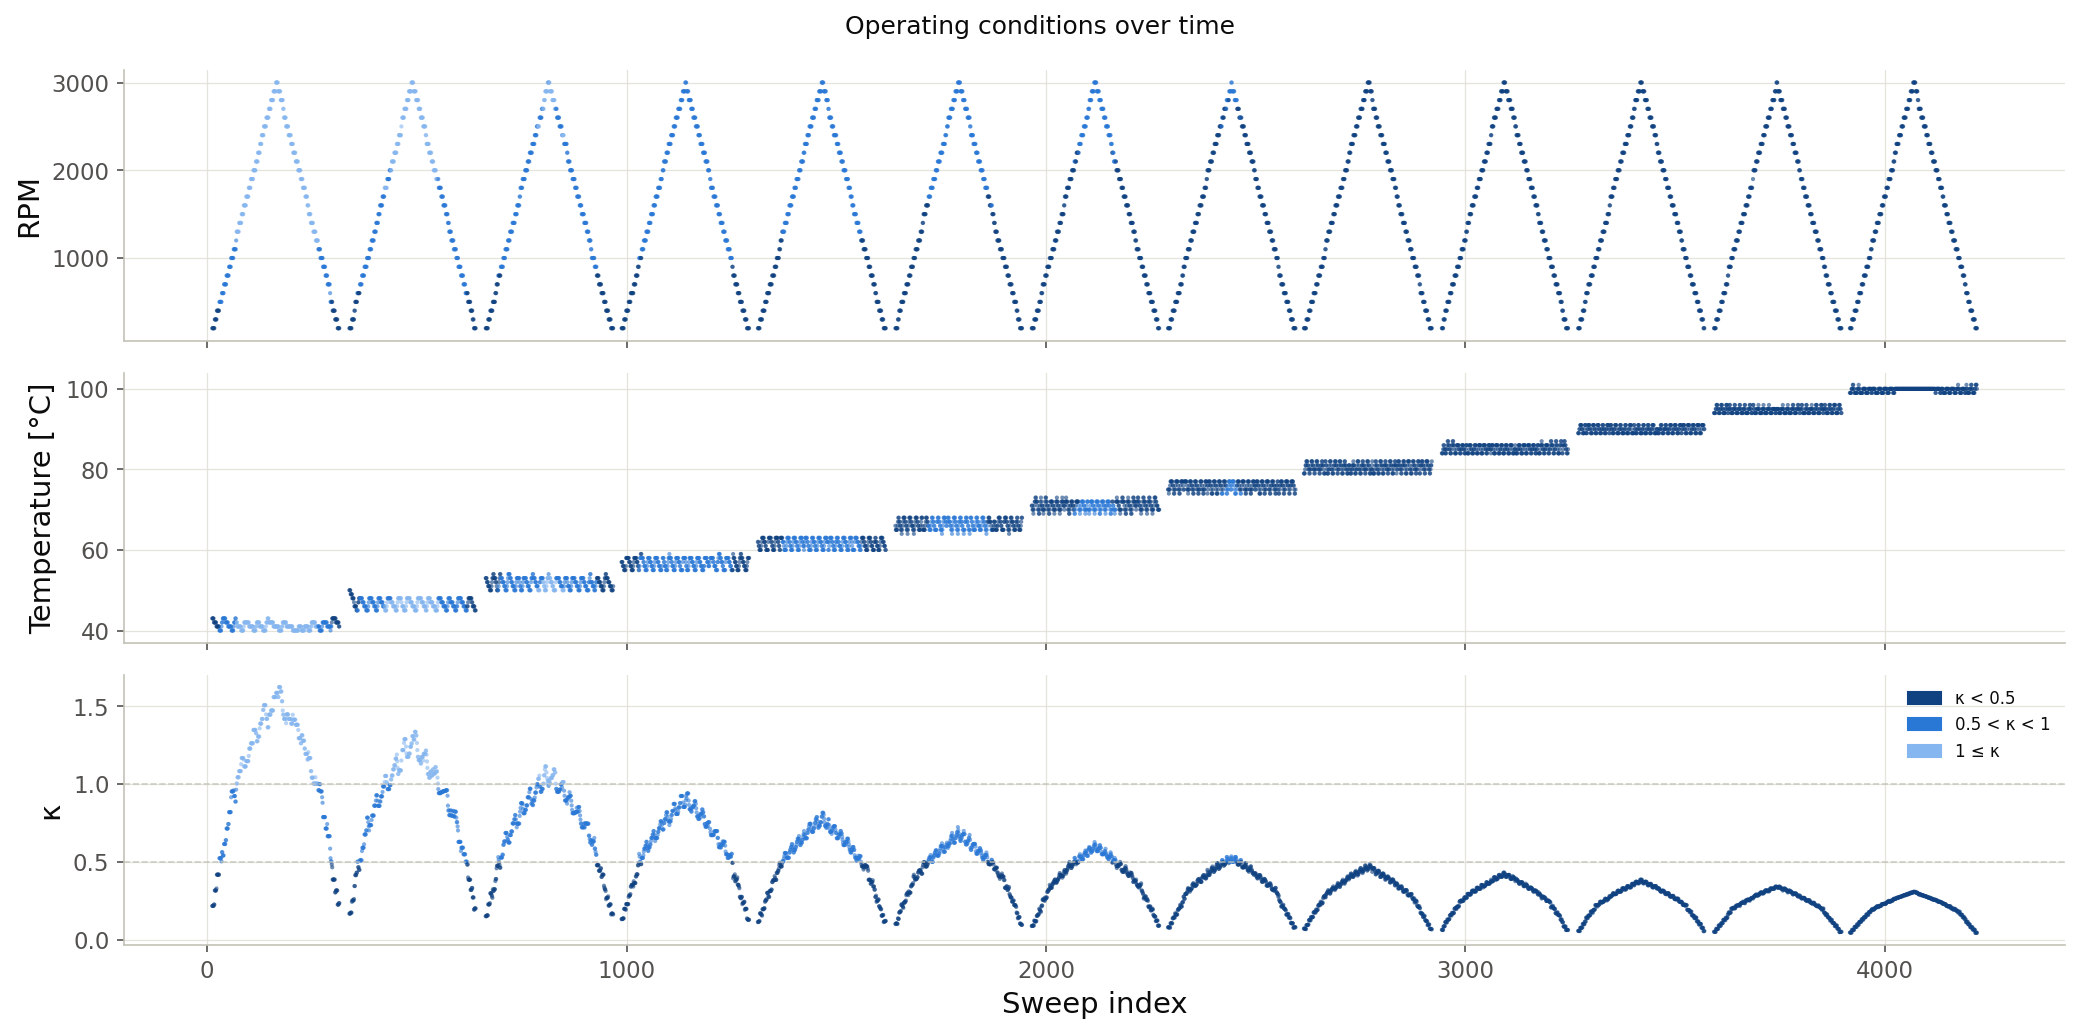
\includegraphics[width=0.9\textwidth]{figures/eda_conditions_timeseries.png}
\caption{Measured operating conditions (RPM and temperature) during the experiment, ordered chronologically by aquisition time. Each point corresponds to a 20ms segment of sampling. The colour of each point corresponds to the derived $\kappa$ value for that segment.}
\label{fig:op_conditions_timeseries}
\end{figure}

\subsection{Sensor configuration and data acquisition}
\label{subsec:sensors}

\subsubsection{Acquisition segments}
Data are acquired as short windows rather than continuously: every
$\sim$\resWindowIntervalS~s the oscilloscope captures a \resWindowMs~ms window
($N \approx 2.5 \times 10^{5}$ samples per channel) containing time-synchronous AE
and US waveforms, together with the mean RPM and housing temperature over the window.
Throughout this paper, one such window is referred to as a \emph{sweep}, and a sweep
is the unit of observation for all feature extraction, model training, and
evaluation. After excluding an initial stationary warm-up segment recorded before the first
staircase, the protocol yields \resNsweepsRaw{} raw sweeps, of which
\resNsweepsRemoved{} with measured RPM above the \SI{3000}{rpm} protocol maximum are
discarded, leaving \resNsweeps{} sweeps per channel (median \resSweepsPerHold{}
sweeps per staircase hold). The resulting $\kappa$ distribution spans
$[\resKappaMin,\, \resKappaMax]$ with mean \resKappaMean{}
(Figure~\ref{fig:op_conditions_distribution}).
